For the detuning series we initially want to lock the laser to the cavity. The lock is set up by using the transmission DC signal as our error signal with an adjustable offset, which is sent through our feedback loop to the laser. This kind of lock is advantageous, because it easy to set up, works well when far detuned and can easily stay locked for large periods of time, for example while recording multiple spectra. A disadvantage is that this lock, compared to a PDH-lock, is sensitive to fluctuations in input power. We lock the laser at an input power of \SI{1}{\milli\watt}. We detune away from cavity resonance simple by changing our locking offset point. This is seen as a decrease in DC level on the oscilloscope, we write down the DC level for every detuning.

The optomechanical induced transparency is performed by using the EOM to generate the weak probe field with the output source from vector network analyzer\footnote{Rohde \& Schwartz ZNB20}, which is then sweept in frequency from \SIrange{0}{10}{\mega\hertz}, i.e. across the cavity response. The sidebands are generated with a source power of \SI{-15}{\deci\bel\milli} and the transmission detector's AC signal is fed as the input to vector network analyzer, but is attenuated by \SI{13}{\deci\bel} to avoid overloading. We record the spectra of the driven cavity response for different detunings from \SI{100}{\kilo\hertz} to \SI{10}{\mega\hertz} with 50 k samples, see an example of such a spectrum in figure \ref{fig:omit_cavity}.

\begin{figure}[H]
\centering
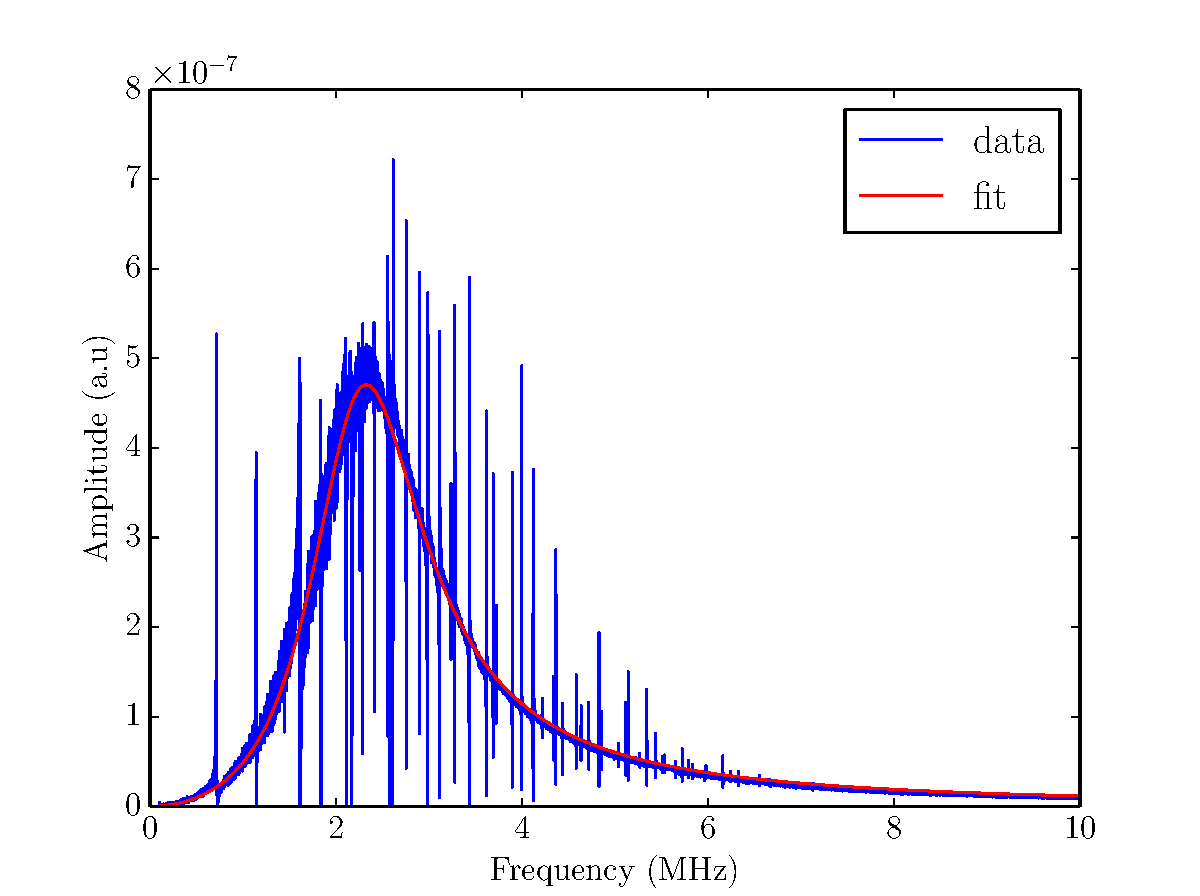
\includegraphics[scale=0.8]{analysis/omit_fit_detuning_new.pdf}
\caption{Example of driven cavity response spetrum from a optomechanical induced transparency measurement. As a rough rule of thumb the cavity response peak frequency is equivalent to the detuning.}
\label{fig:omit_cavity}
\end{figure}

We can obtain the detuning $\bar{\Delta}$ and the cavity linewidth by applying the OMIT model to the normalised response curve. The reasoning behind using the normalised data instead of the raw data, is that amplitude and detuning are not independent, i.e. two different set of values can produce the same curve. Futhermore we set the coupling and mechanical linewidth to zero, so that we only fit to the broad cavity response as shown in figure \ref{fig:omit_cavity}. From the fitting we get the detuning as a function of DC voltage level from the detector see figure \ref{fig:omit_detuning}.

\begin{figure}[H]
\centering
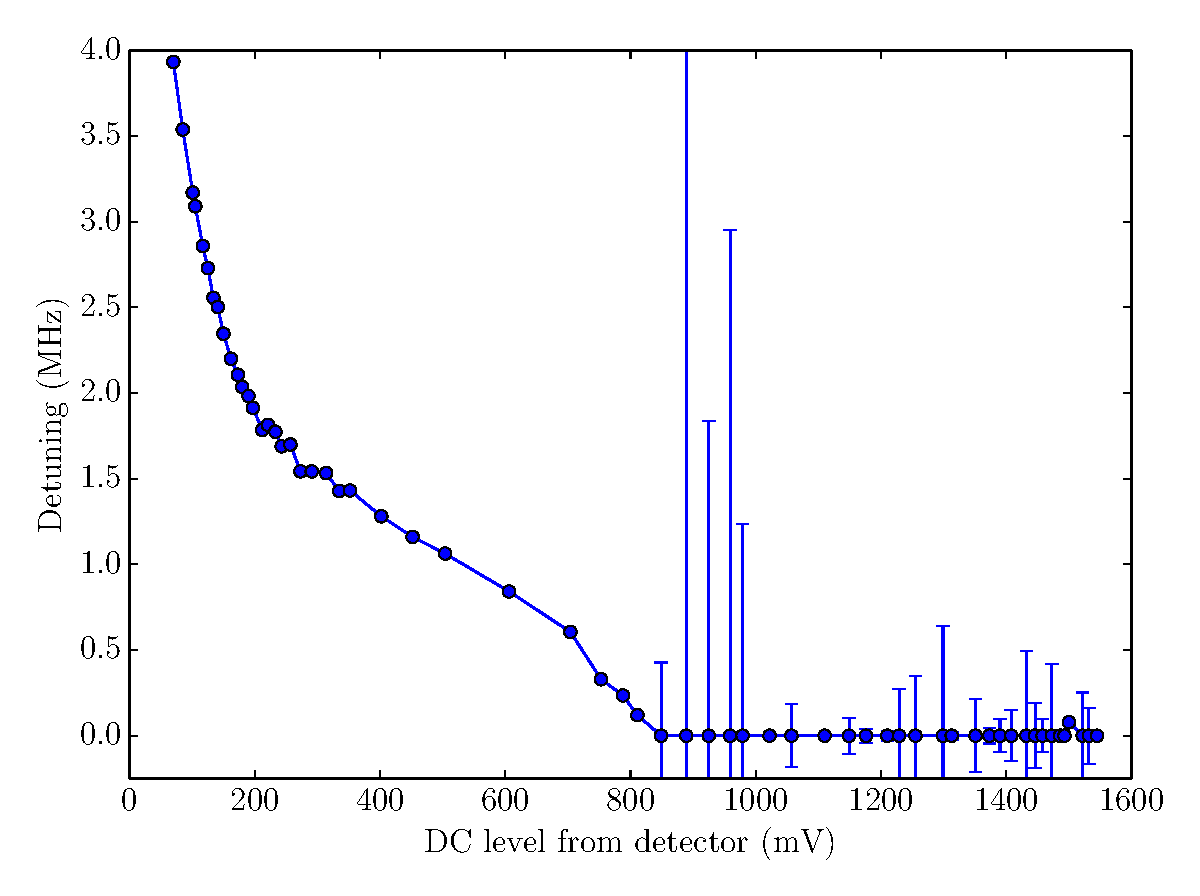
\includegraphics[scale=0.7]{analysis/detuning_vs_DC.pdf}
\caption{The obtained detunings from fitting, showing the detunings for different detector voltages. The uncertainties are the standard deviations from the fit.}
\label{fig:omit_detuning}
\end{figure}

We see from the figure \ref{fig:omit_detuning} that the fit is untrustworthy for small detunings, i.e. detunings lower than \SI{0.5}{\mega\hertz}. Therefore detunings lower than \SI{0.5}{\mega\hertz} will be discarded and that is also acceptable, since we are really only interested in what happens at detunings close to the mechanical frequency, i.e. \SI{2.17}{\mega\hertz} for maximum cooling effects. This is a good time to point out that we do not know our detuning precisely while experimenting, unless we take optomechanical induced transparency traces. We could of course do rough estimates from the Lorentzian cavity line shape, if we know our cavity linewidth. Apropos linewidth we also get this parameter from our fit, see figure \ref{fig:omit_cavity_lw}.

\begin{figure}[H]
\centering
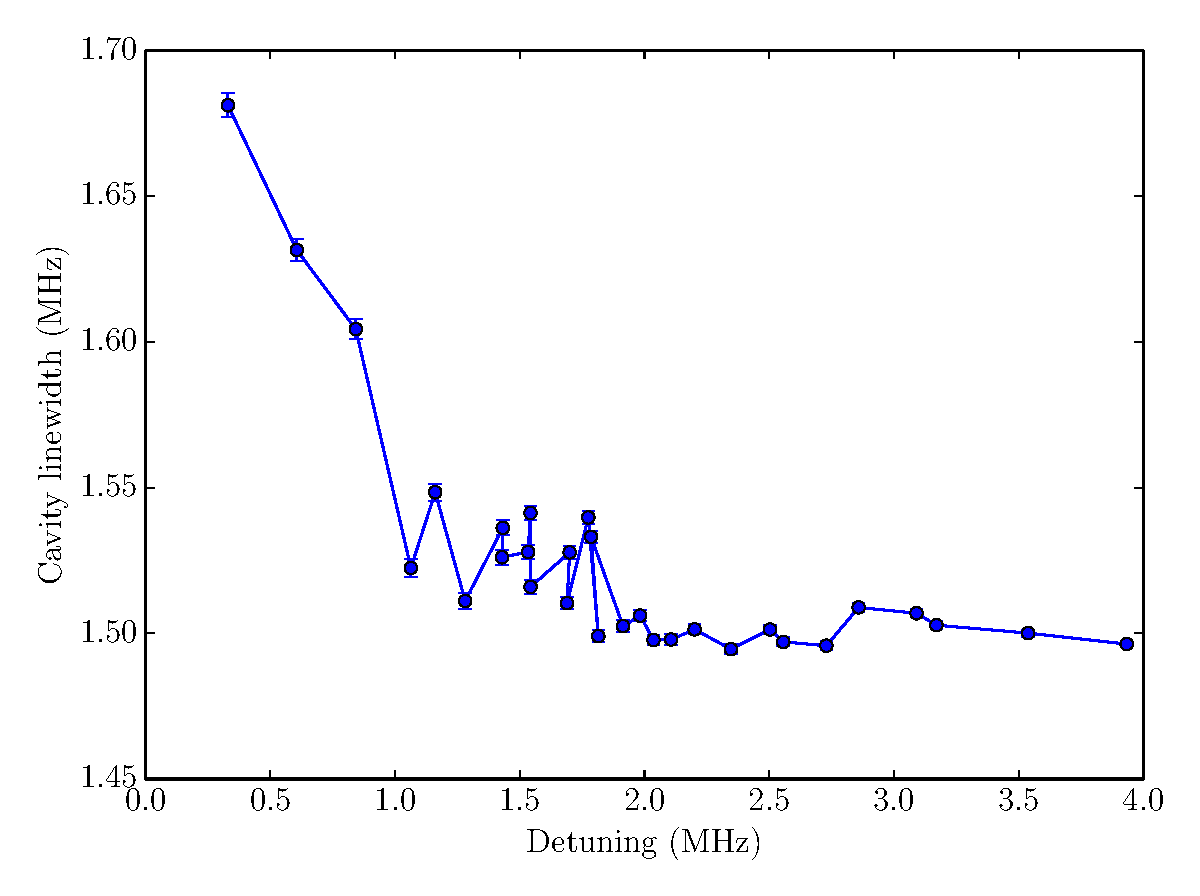
\includegraphics[scale=0.7]{analysis/cavity_lw_vs_detuning_new.pdf}
\caption{Extracted cavity linewidth from the fit to the cavity response. The uncertainties are the standard deviations from the fit.}
\label{fig:omit_cavity_lw}
\end{figure}

We see in figure \ref{fig:omit_cavity_lw} that the cavity linewidth stabilizes for higher detunings. From the optomechanical induced transparency model we get a cavity linewidth of $(1.54 \pm 0.05)$ \SI{}{\mega\hertz}. This result fits well with the independent measured linewidth from section \ref{sec:char_mim}, which is a nice sanity check of our cavity response fit procedure. The rapid increase in cavity linewidth for small detunings is a fitting artifact.

We now turn to fit our model for optomechanical induced transparency at the mechanical frequency (\SI{2.17}{\mega\hertz}) of the (3,3)-mode, i.e. obtaining the light enhanced optomechanical coupling $g = g_0\sqrt{\bar{n}_{cav}}$, where $g_0$ is the single-photon coupling strength defined as $g_0 = Gx_{zpf}$. We perform the fit by choosing a suitable range around the mechanical resonance as seen in figure \ref{fig:omit_g}. The fit parameter $g$ is the width of the dip, while the center of it is the mechanical resonance frequency. The mechanical linewidth is assumed to be zero in our applied model, this is a good assumption because the effective mechanical linewidth will be dominated by the optical induced linewidth.

\begin{figure}[H]
\centering
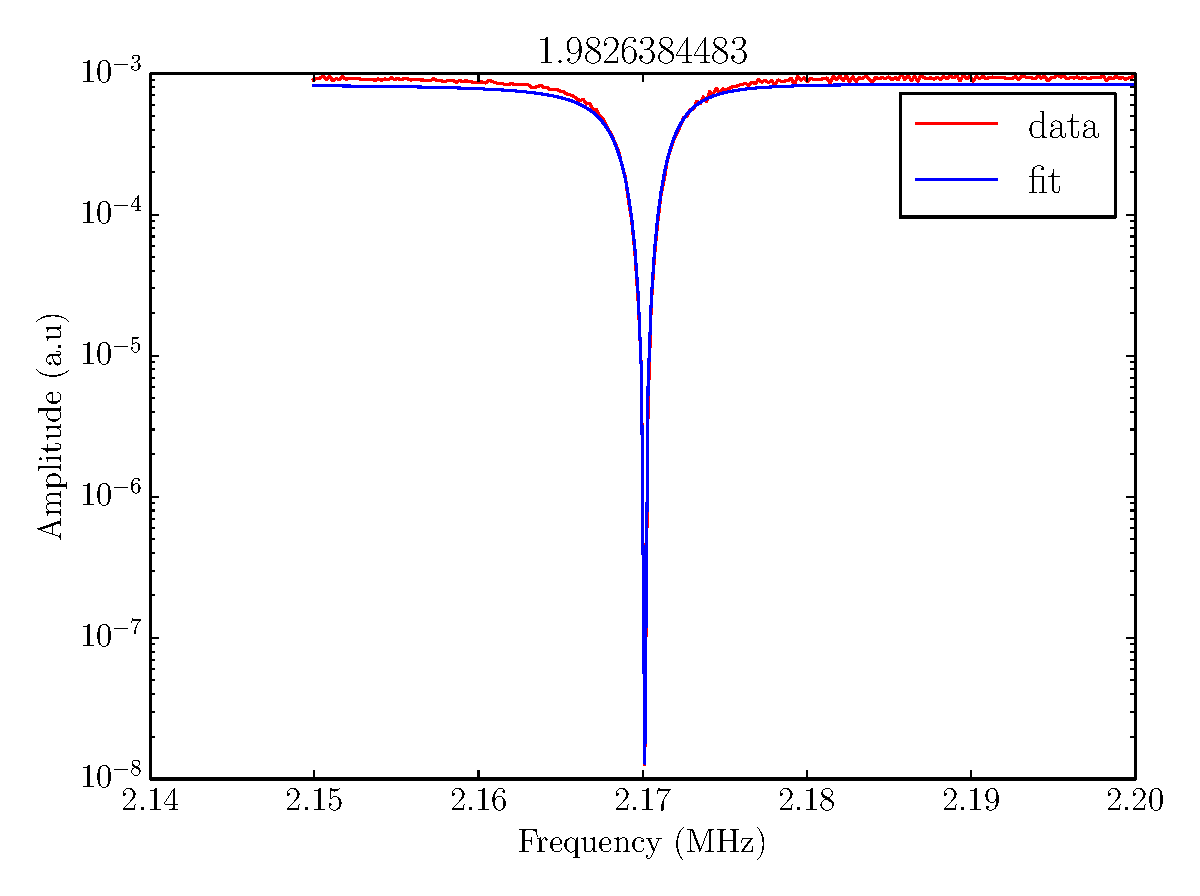
\includegraphics[scale=0.7]{analysis/omit_fit_dip_zoom.pdf}
\caption{Optomechanical induced tranparency. The figure title is the detuning in MHz.}
\label{fig:omit_g}
\end{figure}

We can gain a lot of insight from the fitted parameter $g$, for example $g_0$. If we can work out the intra-cavity photon number, we can obtain $g_0$, which is important for calibrating a spectrum. We can obtain the intra-cavity photon number by using equation \eqref{eq:cav_circ_pwr} and converting the recorded detector DC voltage into an optical power.

\begin{figure}[H]
\centering
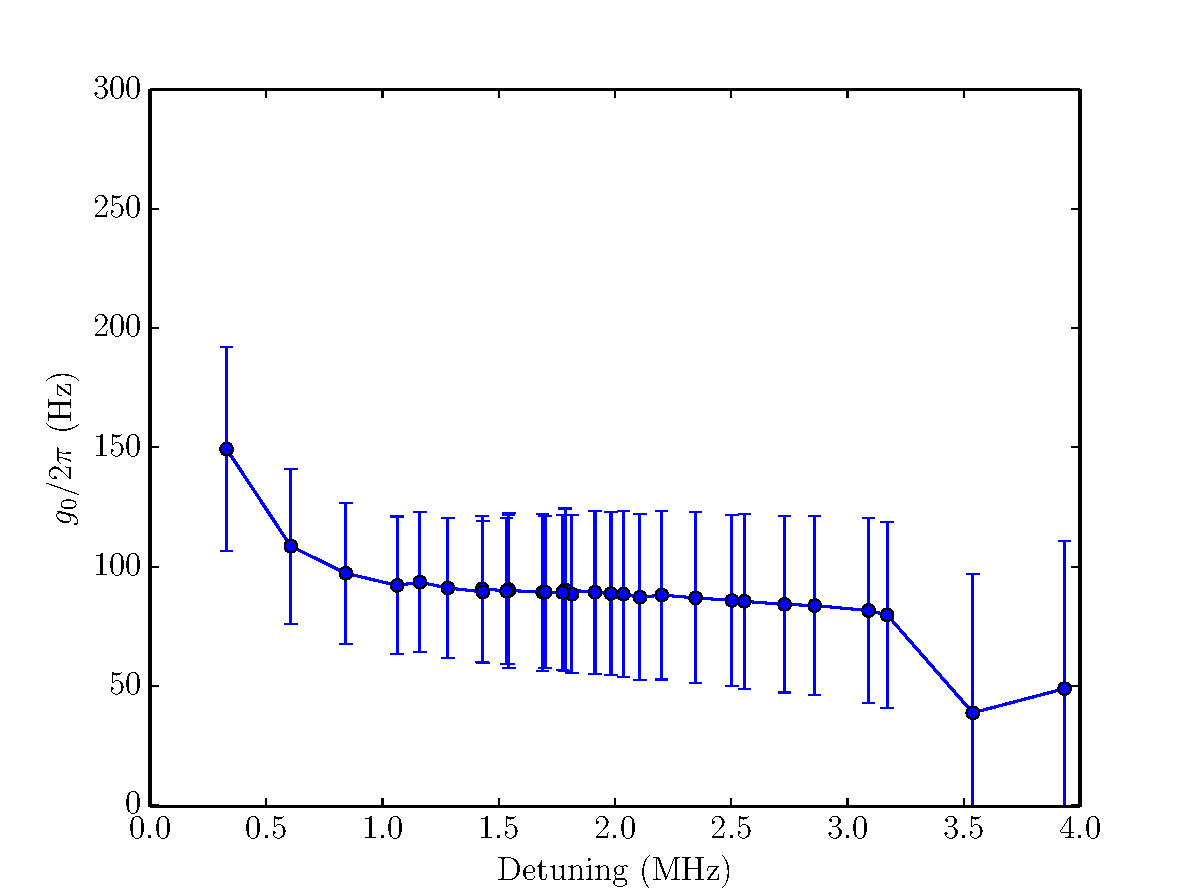
\includegraphics[scale=0.8]{analysis/omit_g0.pdf}
\caption{Single-photon coupling strength as a function of detuning. The errorbars are given by the standard deviation from the fitted $g$.}
\label{fig:omit_fit_g0}
\end{figure}

We get a single-photon coupling strength of $g_0/2\pi = (88.2 \pm 16.8)$ \SI{}{\hertz}. This value of $g_0/2\pi$ sounds reasonable, because a rough estimate of the expected single-photon coupling strength for our parameter set is given by $Gx_{zpf}$. The zero-point fluctuation, using equation \eqref{eq:xzpf}, for the (3,3)-mode is \SI{0.6}{\femto\meter} and if we approximately set $G$ for a Fabry-Perot cavity by $\frac{\omega_c}{L}$, then we should expect \SI{122}{\hertz}. A reduction of $g_0$ is expected from the overlap integral between the beam spot and mechanical mode shape and from the low reflectivity of the membrane \cite{Wilson2011}.

We can also extract the expected optically induced damping $\Gamma_{opt}$ from the cavity resonance by using $g$ and equation \eqref{eq:gamma_opt}. As an approximation we will assume $\Gamma_{opt} \approx \Gamma_{eff}$, since the mechanical linewidth is on the order \SI{}{\hertz} and the optically induced linewidth is on the order \SI{}{\kilo\hertz}. This estimate is shown in figure \ref{fig:omit_fit_gamma_opt}.

\begin{figure}[H]
\centering
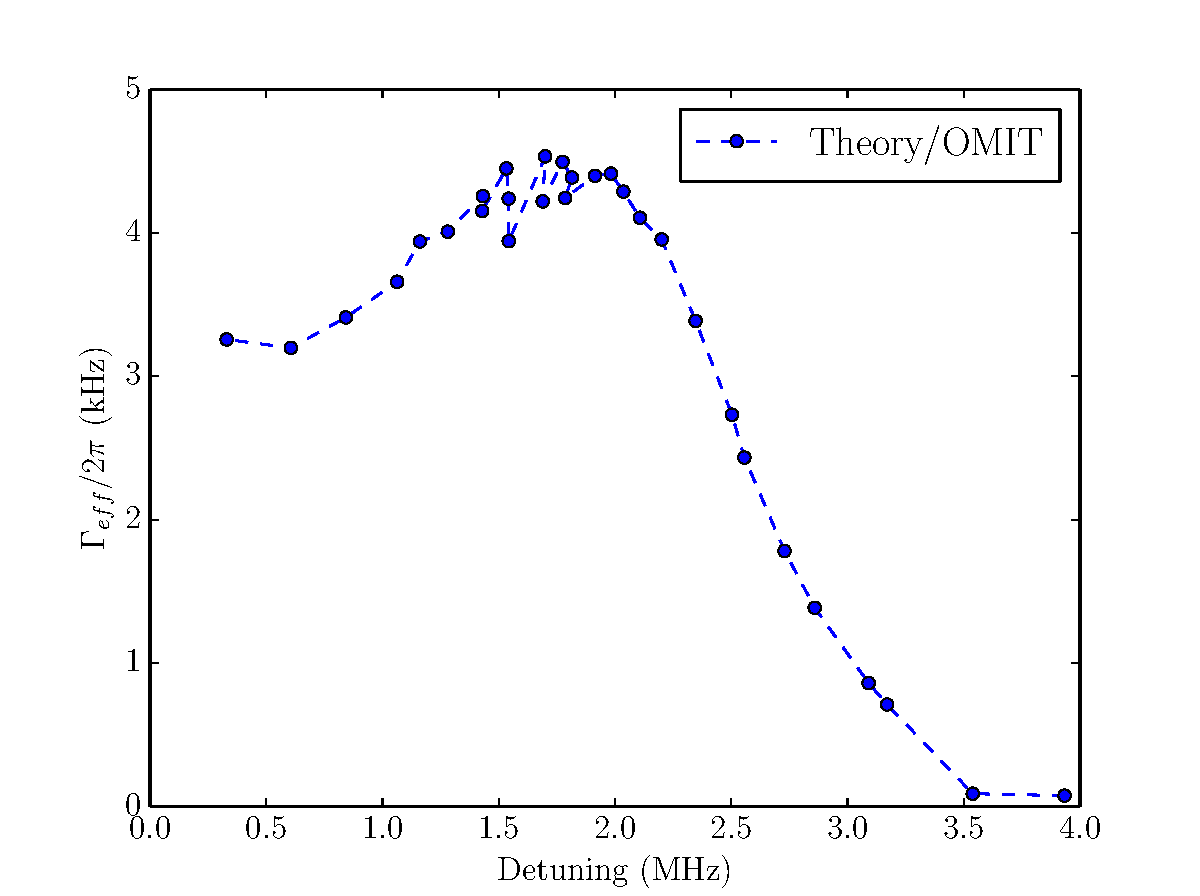
\includegraphics[scale=0.8]{analysis/gamma_opt_vs_detuning.pdf}
\caption{The expected effective mechanical linewidth as a function of detuning.}
\label{fig:omit_fit_gamma_opt}
\end{figure}

We do not know the temperature of the bath that we couple to, so estimating a mean phonon occupancy from the effective damping would not make much sense. The bath temperature can be extracted from the simultaneously recorded spectrum, with a calibraiton peak, of the intensity fluctuations from the cavity caused by the membrane fluctuations, for each individual detuning.